\begin{frame}{Other work done}
    Discontinuous initial condition "Créneau" 
    \begin{equation}
        u_0(x) = \begin{cases}
            A & \text{if } 0.40 \leq x \leq 0.50, \\
            B & \text{otherwise},
        \end{cases}
    \end{equation}

    By training our NN with $A$ varying beetween $0.6$ and $0.7$ and $B=0.3$ fixed, 
    epochs $= 20.000$, collocation $= 0$, data$=10000$ and $A=0.66$ we obtained:

    
    \begin{figure}
        \centering
        
        \begin{subfigure}{0.32\textwidth}
            \centering
            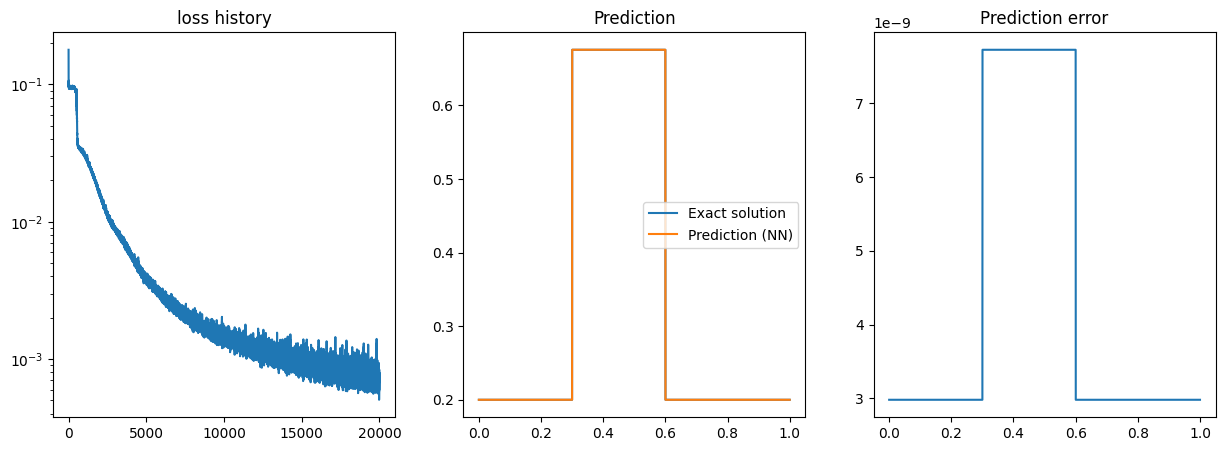
\includegraphics[width=\textwidth]{images/c1.png}
            \caption{t=0}
        \end{subfigure}
        \begin{subfigure}{0.32\textwidth}
            \centering
            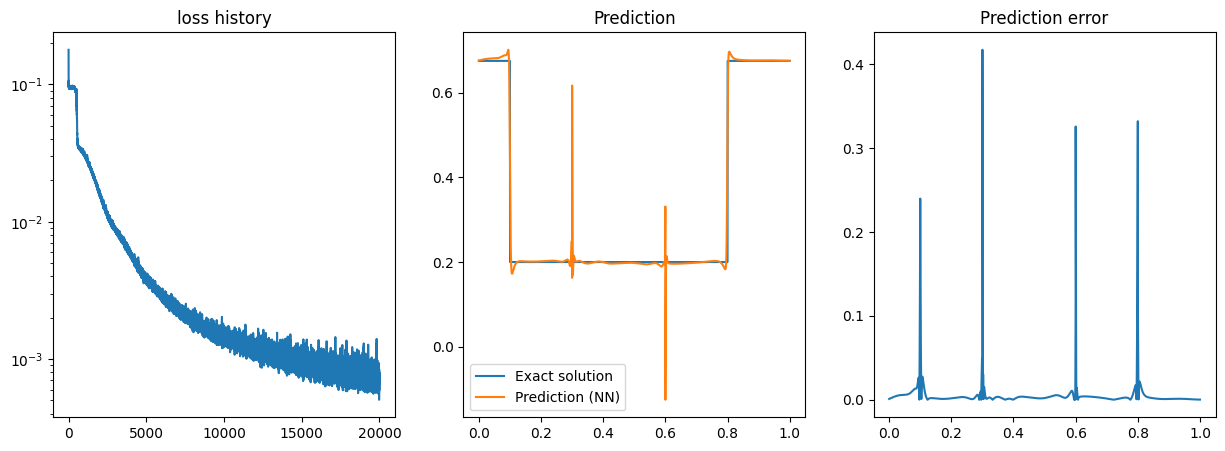
\includegraphics[width=\textwidth]{images/c2.png}
            \caption{t=0.5}
        \end{subfigure}
        \begin{subfigure}{0.32\textwidth}
            \centering
            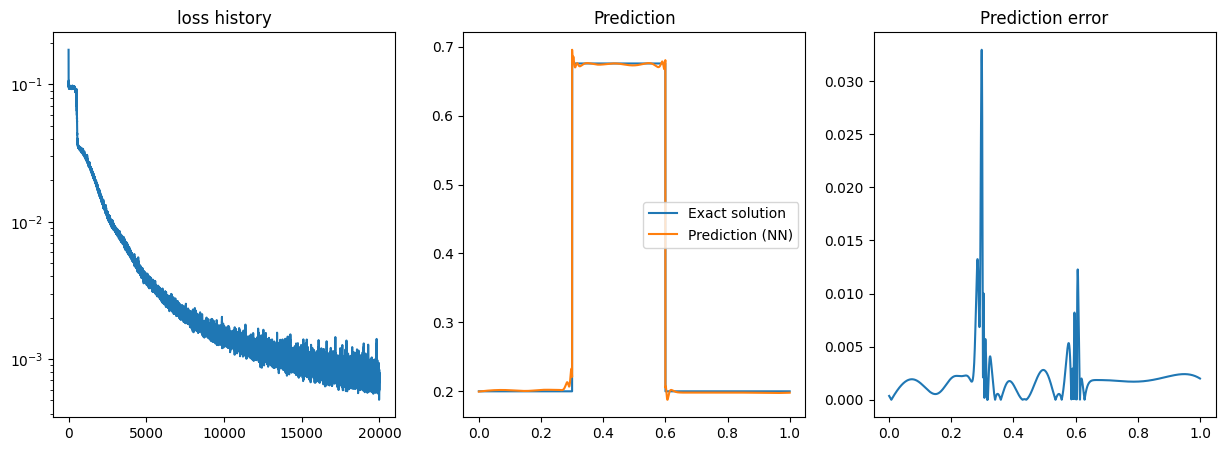
\includegraphics[width=\textwidth]{images/c3.png}
            \caption{t=1}
        \end{subfigure}
    \end{figure}


\end{frame}
